\documentclass[12pt, a4paper]{article} %,fleqn
\usepackage{Diplo}

\usepackage[left=3cm,right=3cm,
top=2cm,bottom=2cm]{geometry}



\usepackage{comment}
\usepackage{hyperref}
\usepackage{dsfont}
\newtheorem{definition}{Определение}
\newtheorem{theorem}{Теорема}
\newtheorem{utv}{Утверждение}

\graphicspath{{../pics/}}


\begin{document}
	
\vskip 3mm

\setcounter{page}{1}
%%%%%%%% Титульный лист %%%%%%%%%%%%%%%%%%%%%%%%%%%%%%%%%
\begin{center}
	\thispagestyle{empty}
	
	{ Министерство науки и высшего образования Российской Федерации\\}

	
	
	{ Московский Физико-технический институт \\}
	
	{ (Государственный Университет) \\}
	
	{ Факультет управления и прикладной математики  \\}
	
	{ Кафедра Интеллектуальных систем\\}
	
	{при Вычислительном Центре им. А.А.Дородницына РАН\\ [4cm]}
	
	{ \bf \Large Выпускная квалификационная работа\\}
	
	{ \bf \Large{"Разработка и реализация нейросетевой системы для извлечения именованных сущностей генов и мутаций из медицинских текстов"\\[1cm]} }
	
	{\bf {Студента 4-го курса Сотникова Антона Дмитриевича}\\[3cm]}
	
\end{center}

\begin{flushright}
	\bf{Научный руководитель}\\
	\bf{д.т.н., Дулин С.К.}\\[0.5cm]
\end{flushright}

\begin{flushright}
	\bf{Научный консультант}\\
	\bf{д.т.н., Хорошевский В.Ф.}\\[2cm]
\end{flushright}



\begin{center}
	Москва, 2020
\end{center}
%%%%%%%%%%%%%%%%%%%%%%%%%%%%%%%%%%%%%%%%%%%%%%%%%%%%%%%%%%%%%%%%

\newpage
\begin{abstract}
	Решается задача распознавания именованных сущностей генов и мутаций в биомедицинских текстах. Предлагается система GMNet, основанная на рекуррентных нейронных сетях с использованием двунаправленной долгой краткосрочной памяти и условных случайных полей. Модель получает на вход последовательность токенов и на выходе определяет класс каждого токена. GMNet обучается на нескольких данных, находящихся к открытом доступе. Система, представленная в данной работе, достигает 80.34\% и 87.09\% по F-мере для сущностей генов и мутаций, соответственно, что является соизмеримым с результатами существующих моделей и приводит к выводу о ее высокой производительности при решении задачи извлечения именованных сущностей из медицинских текстов. 
	
	\bigskip
	\textbf{Ключевые слова:} \textit{распознавание именованных сущностей, рекуррентные нейронные сети, случайные условные поля, гены и мутации.}
\end{abstract}


\newpage
\tableofcontents
 


\newpage
\section{Введение}
%Общие слова
В настоящее время наблюдается значительный рост биомедицинских исследований и связанных с ними публикаций. Поэтому извлечение важной и ценной информации из них становится всё более сложной задачей. Исследователи проделывают серьёзную работу по поиску источников информации о биологических и медицинских сущностях, их структуризации и дальнейшей разметки \cite{Galea2018a}. Всё это делается для повышения качества новых исследований. Технически, поиск имен генов и мутаций является поиском именованных сущностей в тексте (NER), но существует ряд обстоятельств, сильно усложняющих решение такой задачи: огромное число генов и мутаций, которое растет с каждым днем; не существует единой записи подобных сущностей -- они могут быть записаны в стандартном (\textit{g.3912G>C}), полустандартном форматах (\textit{3992-9g–>a mutation}) или полностью на естественном языке (\textit{deletion of 10 and 8 residues from the N- and
C-terminals}). Также названия генов и мутаций могут встречаться в тексте и с другими биомедицинскими сущностями, которые имеют сходную морфологию и сходный контекст. Все это делает поиск рассматриваемых сущностей трудной и важной задачей.  Именно поэтому так важно создавать быстрые и точные методы обработки естественного языка и анализа биомедицинской литературы, чтобы извлекать полезную информацию из возрастающего потока данных.

	 

\bigskip

\textbf{Цели и задачи данной работы.} Основной целью исследования является построение модели на основе рекуррентных нейронных сетей и достижения после её реализации соизмеримого или более высокого качества выделения именованных сущностей генов и мутаций по сравнению с уже существующими моделями. Для реализации этой цели были поставлены следующие задачи:
\begin{itemize}
	\item изучить существующие подходы к решению задачи извлечения именованных сущностей генов и мутаций;
	\item провести поиск существующих размеченных корпусов, пригодных для задач машинного обучения, для решения этой задачи;
	\item определить пригодность найденных источников данных;
	\item провести предобработку данных;
	\item реализовать основные алгоритмы и архитектуру нейронной сети;
	\item модернизировать модель путем обучения дополнительных векторных представлений для каждого символа с целью увеличения информации о токенах, не входящих в словарь (Out Of Vocabulary problem);
	\item реализовать модернизированную модель, обучить её на имеющихся данных, провести поиск оптимальных гиперпараметров;
	\item провести вычислительный эксперимент и получить значения метрик качества.
\end{itemize}

\bigskip

\textbf{Научная новизна.} Используется новый подход в решении задачи извлечения именованных сущностей генов и мутаций из медицинских текстов, основанный на использовании контекстной информации с помощью рекуррентных нейронных сетей.

\bigskip

\textbf{Методы исследования.} Использованы методы машинного обучения и нейронных сетей, методы классификации отдельных лексем (токенов) в текстах.

\bigskip

\textbf{Практическая ценность.} Полученная модель может быть использована в качестве встраиваемого модуля в более общие модули. Например, с её помощью можно решать следующие задачи.
\begin{enumerate}
	\item Строить временные ряды по интересам авторов по разным генам и мутациям. Это дает тренды в данной области и позволяет делать предположения о том, где искать новые применения полученным знаниям.
	\item Строить вопросно-ответные системы с целью диагностики симптомов заболевания, вызванного той или иной генетической мутацией.	
\end{enumerate}

\bigskip

Работа состоит из пяти разделов, заключения и списка литературы. Содержание изложено на 2 страницах. Список литературы включает 26 наименования.

Во \textbf{Введении} обосновываются цели и задачи исследования, его научная и практическая значимость.

В \textbf{Разделе 2} формулируется постановка задачи, а также используемые для оценки ее решения показатели качества.

В \textbf{Разделе 3} приводится анализ существующих методов решения задачи извлечения именованных сущностей генов и мутаций из биомедицинских текстов.

В \textbf{Разделе 4} описывается архитектура предлагаемой в работе модели.

В \textbf{Разделе 5} описываются используемые данные, параметры обучения модели, вычислительный эксперимент и анализ полученных результатов.

В \textbf{Заключении} фиксируются основные результаты работы и указываются направления дальнейших исследований.

%%%%%%%%%%%%%%%%%%%%%%%%%%%%%%%%%%%%%%%%%%%%%%%%%%%%%




\newpage
\section{Постановка задачи}
Для определения меток генов и мутаций в задаче рассматривается подход \textbf{sequence labeling} (разметки последовательности), являющийся в данном случае обобщением метода классификации. Рассматриваются множество $\mathcal{K}$, состоящее из 5 классов (меток, тэгов) -- \textsc{o, b-gene, i-gene, b-mut, i-mut}, где префиксы B и I означают начало (begin) и внутренние составляющие (inside) именованной сущности, а O -- остальное (other).
\subsection{Формальная постановка задачи}


Дана выборка и множество меток $$\mathcal{D} = \left\{\mathbf{x}_i, \mathbf{{y}_i}\right\}_{i=1}^N, ~~~ \mathcal{K}=\left\{\mathit{{k}_j}\right\}_{j=1}^5,$$ где $\mathit{x}_i\in \mathbb{R}^{n_i}$~-- последовательность токенов в предложении длины $\mathit{n}_i$, ${y}_i \in \mathbb{R}^{n_i}$~-- соответствущая им последовательность меток, а $k_j\in \left[\textsc{o, b-gene, i-gene, b-mut, i-mut}\right]$.

Требуется построить модель
	$$\mathit{a} : (\mathbf{w}, \mathbf{X})\rightarrow\mathbf{y},$$
	где	$\mathbf{w} \in \mathbb{W}$~-- параметры модели, $\mathbf{X} = \bigcup_{i=1}^N\bigcup_{j=1}^{n_i} \mathit{x}_j, \mathbf{y} = \bigcup_{i=1}^N\bigcup_{j=1}^{n_i} \mathit{y}_j$.

Функция ошибки
	$$\mathcal{L}\left(\mathbf{y}, \mathbf{X}, \mathbf{w}\right)=-\sum_{i=1}^{N}\log(\mathbb{P\{\mathbf{y_{ik}}|\mathbf{x_{i}}\}}).$$

Решается задача оптимизации: 
	$$\textbf{w}^* = \underset{\mathbf{w}\in\mathbb{W}}{\text{argmin}} ~ \mathcal{L}(\textbf{w}).$$

 

\subsection{Показатели оценки качества}
Для оценки качества классификации токенов в задаче NER используются метрики \textit{Precision, Recall, F1-measure} \cite{Chinchor1993}. Для их вычисления вводятся следующие обозначения:
\begin{itemize}
	\item \textbf{Correct (COR)} -- совпадение метки;
	\item \textbf{Incorrect (INC)} -- несовпадение метки;
	\item \textbf{Partial (PAR)} -- границы прогнозируемой сущности перекрываются с ground-truth границами;
	\item \textbf{Missing (MIS)} -- сущность не была найдена;
	\item \textbf{Spurius (SPU)} -- сущность была найдена неверно.
\end{itemize}

Далее вводятся число всех возможных сущностей в корпусе
$$\textit{Possible(POS)}=\textit{COR} + \textit{INC} + \textit{PAR} + \textit{MIS}=\textit{TP} + \textit{FN}$$
и число сущностей, предсказанных моделью
$$\textit{Actual(ACT)}=\textit{COR} + \textit{INC} + \textit{PAR} + \textit{SPU}=\textit{TP} + \textit{FP}.$$

Возможны два сценария расчета метрик точности и полноты в зависимости от учета предсказанных границ именованных сущностей.

\textbf{Строгое соответствие} не учитывает те предсказания, которые полностью не совпадают с ground-truth границами. В таком случае метрики принимают вид

$$\textit{Precision}=\frac{\textit{COR}}{\textit{ACT}}=\frac{\textit{TP}}{\textit{TP}+\textit{FP}}, ~~~~~~ \textit{Recall}=\frac{\textit{COR}}{\textit{POS}}=\frac{\textit{TP}}{\textit{TP}+\textit{FN}}.$$ 

\textbf{Частичное совпадение} штрафует за несовпадение границ, однако учитывает, что сущность была обнаружена почти верно:

$$\textit{Precision}=\frac{\textit{COR}+0.5\cdot\textit{PAR}}{\textit{ACT}}, ~~~~~~ \textit{Recall}=\frac{\textit{COR}+0.5\cdot\textit{PAR}}{\textit{POS}}.$$

Зная значения точности и полноты для предсказаний модели, можно посчитать их среднее гармоническое:
$$\textit{F-measure}=\frac{2\cdot\textit{Precision}\cdot\textit{Recall}}{\textit{Precision}+\textit{Recall}}.$$

В данной работе предлагается использовать сценарий строгого соответствия.	



%%%%%%%%%%%%%%%%%%%%%%%%%%%%%%%%%%%%%%%%%%%%%%%%%%%%%

\newpage
\section{Обзор существующих методов}
В данном разделе будут более подробно рассмотрены конкретные методы, с помощью которых решалась рассматриваемая задача. 

%Задача NER
Прежде всего нужно определить термины, которые являются наиболее ценными для проводимого исследования. Такие термины называются именованными сущностями, а задача по их нахождению (Named Entity Recognition, NER) является одной из самых важных для автоматического поиска этих объектов в тексте и дальнейшей их классификации к определённым типам. Чаще всего задача NER является первым этапом в решении более общих задач, например, при поиске отношений между сущностями или построении вопросно-ответных систем, так как она позволяет получить ценную информацию из текстов, что существенно помогает в исследованиях. В биомедицине наибольший интерес представляют именованные сущности генов, белков, их мутаций, химических соединений, а также заболеваний \cite{Zhu2018}. Тем не менее, задача NER в биомедицинских текстах является довольно сложной, так как объекты могут состоять из смеси различных символов или нескольких слов. Кроме того, имеют место сокращения и синонимы. Для ее решения существуют два подхода: на основе обучения по прецедентам и без учителя. 

\subsection{Методы обучения без учителя}
\subsubsection{Методы, основанные на словарях}

%Кратко о подходах и их недостатках
Первые подходы к решению задачи NER в области биомедицины основывались на использовании правил и словарей (rule-, vocabulary-based подходы) \cite{UlfLeser2005}. Использование словарного метода подразумевает составление некоторого исходного словаря, на основе которого происходит извлечение биологических сущностей из текста. 

Так, в \cite{Krauthammer2001} предлагается использовать следующий подход. Имена генов выгружаются из банка названий генов и белков, который являлся словарем. 
\begin{figure}[h]
	\center{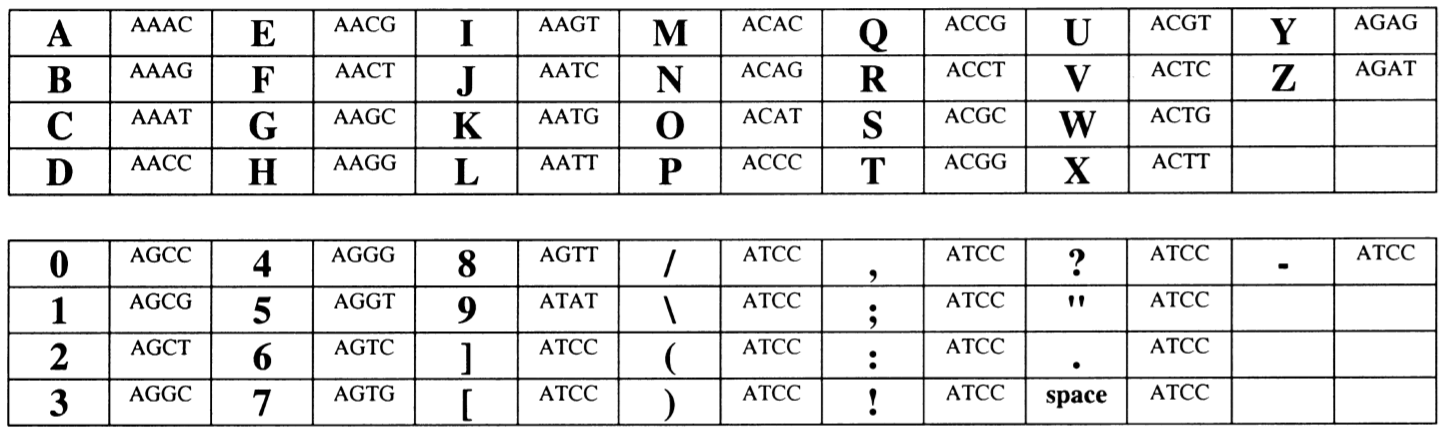
\includegraphics[width=0.6\linewidth]{blast.png}}
	\caption{Таблица перевода в нуклеотидные цепочки.}
	\label{ris:image1}
\end{figure}
Далее, часть слов фильтруется за исключением часто встречающихся анлийских слов и записей, состоящих только из цифр. Затем имена преобразовываются в нуклеотидные последовательности путем замены каждого символа заранее определенной уникальной нуклеотидной комбинацией с помощью специальной таблицы без учета регистра. Используя такую же процедуру, в такой формат переводятся и медицинские тексты, после чего находятся полные и частичные соответствия между закодированными генами и текстом.

\subsubsection{Методы, основанные на правилах}
Модели, использующие rule-based подходы, распознают именованные сущности по заранее написанным правилам, определяющимся по текстовым шаблонам. 

В \cite{Hanisch2005} используется предобработанный словарь синонимов для извлечения потенциальных вхождений имен генов в текстах. Такой словарь связывает каждую биологическую сущность со всеми известными синонимами. После этого, на основе прописанных правил, эта система применятеся для обнаружения всевозможных вхождений имен генов на основе созданного словаря. Для устранения неоднозначности найденных совпадений генов в тексте обнаруживаются имена из внешних словарей. Эти внешние словари содержат сокращения, названия организмов, типы клеток и другие биологические объекты.

Система для ивзлечения мутаций описана в \cite{Caporaso2007} и называется \textit{MutationFinder}. Она использует регулярные выражения для идентификации названия мутации. Метод работает следующим образом: происходит разбиение текста на предложения, затем применяются регулярные выражения к каждому из них. Используя такой подход, становится возможным извлекать сущности мутаций, написанных на естественном языке. Прямым улучшением \cite{Caporaso2007} является работа \cite{Thomas2016}. В ней рассматривается модель \textit{SETH}, использующая следующие четыре модуля: номенклатура человеческих мутаций, регулярные выражения, модифицированный \textit{MutationFinder}, а также литеральные упоминания. \textit{SETH} может объединять найденные несколькими модулями мутации для разрешения неоднозначных ситуаций. Так, например, один модуль может обнаружить подстроку мутации, в то время как номенклатура находит полное упоминание о ней.

\bigskip

Подобные методы показали себя довольно надёжными и производительными и позволили сильно продвинуться в решении рассматриваемой задачи. Но есть существенный недостаток: они сильно зависят от созданных вручную словарей и правил, которые, в свою очередь, зависят от внешних знаний, орфографических особенностей и не являются исчерпывающими для многих видов именованных сущностей.


\subsection{Методы обучения с учителем}
\subsubsection{Модели, основанные на машинном обучении}
Методы, основанные на обучении с учителем, используют размеченные данные для извлечения именованных сущностей. Точность и аккуратность разметки должны быть очень высокими, чтобы алгоритм смог правильно предсказывать метки именованных сущностей.
Для устранения недостатков прошлых методов традиционные подходы к решению задачи NER были заменены на алгоритмы машинного обучения. В таких алгоритмах NER рассматривают как задачу маркировки последовательности, целью которой является нахождение наилучшей последовательности меток для входного предложения.

Так, в работе \cite{pmid28200120} были применены скрытые марковские модели и модели максимальной энтропии в качестве классификаторов для нахождения именованных сущностей генов и мутаций. Методы принимают на вход векторные представления слов, из которых состоит текущее предложение, затем каждому слову ставится в соответствие метка принадлежности к определенному классу. Но такие модели имеют существенный недостаток, называемый ``смещением метки'', суть которого заключается в том, что модель отдает предпочтение меткам с большей энтропией, из-за чего начинает накапливаться ошибка.

В \cite{pmid23564842} было показано, что модель условных случайных полей (Conditional Random Fields, CRF) лишена такого недостатка. В этой публикации, помимо использования стандартных регулярных выражений, в качестве основного идентификатора был выбран классификатор на основе CRF. Это дало значительный прирост в полноте предсказанных сущностей. 

\bigskip

Хотя большинство подходов, основанных на машинном обучении, привели к серьёзным улучшениям в решении задачи извлечения именованных сущностей генов и мутаций из медицинских текстов, они до сих пор остаются зависимыми от заранее описанных функций и человеческого труда.

%О подходе DL
\subsubsection{Модели, основанные на глубоком обучении}
Подходы, основанные на применении глубокого обучения и нейронных сетей \cite{DBLP:journals/corr/LampleBSKD16}, в последнее время всё чаще привлекают внимание исследователей, так как они показывают лучшую производительность в решении таких задач обработки естественного языка, как построение языковых моделей, распознавание речи и машинный перевод. В задаче извлечения именованных сущностей также наблюдается высокий прирост в качестве при использовании нейронных сетей \cite{DBLP:journals/corr/LampleBSKD16}. Так, в публикациях \cite{pmid32046638, Habibi2017, Yoon2019, Weber2019} показана высокая эффективность моделей, использовавших долгую краткосрочную память (Long Short-Term Memory, LSTM) \cite{Hochreiter1997} и условные случайные поля. На вход моделей принимаются векторные представления слов (эмбеддинги), предобученные на большом объеме специализированных под предметную область текстов. Далее, эмбеддинги подаются в LSTM слой, после чего классификатор CRF присваивает очередному слову метку. Такая архитектура позволила использовать контекстную информацию и показывает наилучшие результаты по извлечению именованных сущностей и по сей день. В работе \cite{Zhu2018} предлагается использовать сверточные нейронные сети вместо слоя LSTM. Результаты оказались сравнимыми с предыдущими моделями. На сегодняшний день лучший результат демонстрирует модель BioBERT, описанная в \cite{Lee2019}. Она основана на классической модели \cite{Devlin2019} и дообучена на большом объеме биомедицинских научных статей. BioBERT опережает по F-мере почти все существующие модели, но требует для обучения огромных вычислительных ресурсов. 

Так как именно нейросетевые подходы имеют наилучшую производительность на сегодняшний день, в данной работе предлагается реализовать систему, основанную на использовании методов глубокого обучения.



%%%%%%%%%%%%%%%%%%%%%%%%%%%%%%%%%%%%%%%%%%%%%%%%%%%%%

\newpage
\section{Описание модели}
\subsection{Долгая краткосрочная память}
Рекуррентные нейронные сети (RNN) были разработаны специально для работы с последовательной информацией (рис.1а) \cite{DBLP:journals/corr/LampleBSKD16}. На каждой итерации RNN получает на вход очередное векторное представление слова $\mathbf{x_{i}}$. Далее на основе предыдущего внутреннего состояния $\mathbf{h_{i-1}}$ и $\mathbf{x_{i}}$ формируется выход $\mathbf{y_{i}}$ и новое внутреннее состояние $\mathbf{h_{i}}$. Таким образом, одна и та же матрица весов $\mathbf{W}$ последовательно применяется к очередному элементу входа, что позволяет хранить информацию о контексте каждого слова. Хотя такая модель является довольно производительной, все же она страдает от проблемы затухания и взрыва градиента \cite{DBLP:journals/corr/LampleBSKD16}.	

\begin{figure}[h]
	\begin{minipage}[h]{0.49\linewidth}
		\center{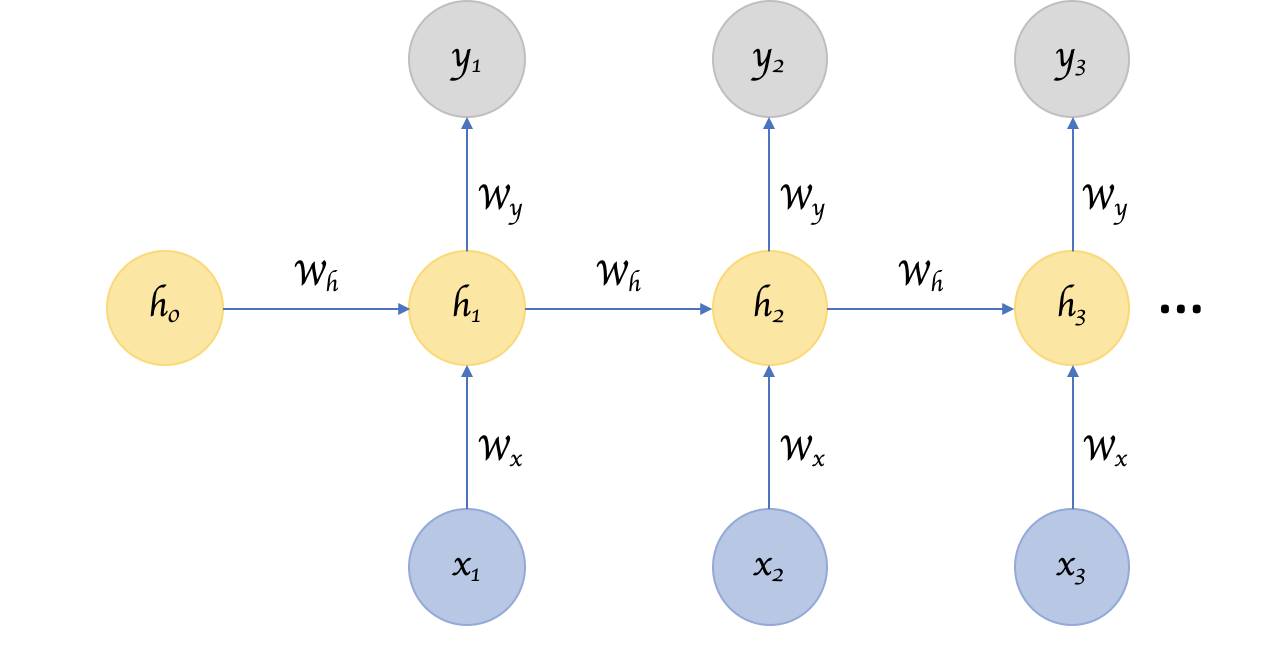
\includegraphics[width=1.1\linewidth]{rnn.png} \\ а)}
	\end{minipage}
	\hfill
	\begin{minipage}[h]{0.49\linewidth}
		\center{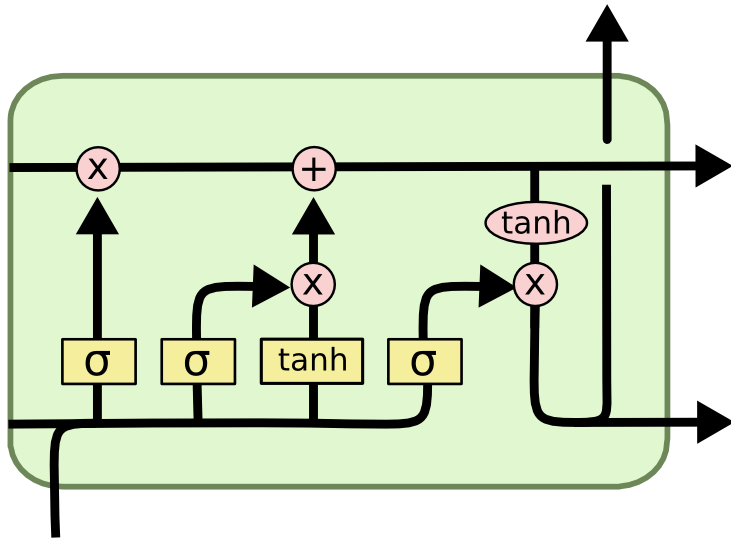
\includegraphics[width=0.78\linewidth]{lstm.png} \\ б)}
	\end{minipage}
	\caption{(a) Пример архитектуры RNN, (б) Архитектура ячейки LSTM.}
	\label{ris:image2}
\end{figure}

Долгая краткосрочная память (LSTM) \cite{Hochreiter1997} помогает в сохранении информации и решает основные проблемы классических RNN. Ячейка такой памяти состоит из трёх фильтров: фильтр забывания информации, фильтр обновления информации и выходной фильтр (рис.1б).
Ниже приведены вычисления, происходящие внутри ячейки LSTM:
\begin{flushleft}


$\hspace{45mm}\mathbf{i}_t=\mathbf{\sigma}(\mathbf{W}_{xi}\mathbf{x}_{t}+\mathbf{W}_{hi}\mathbf{h}_{t-1} + \mathbf{W}_{ci}\mathbf{c}_{t-t} + \mathbf{b}_{i})$

$\hspace{45mm}\mathbf{f}_t=\mathbf{\sigma}(\mathbf{W}_{xf}\mathbf{x}_{t}+\mathbf{W}_{hf}\mathbf{h}_{t-1} + \mathbf{W}_{cf}\mathbf{c}_{t-t} + \mathbf{b}_{f})$

$\hspace{45mm}\tilde{\mathbf{c}}_t = \textit{tanh}(\mathbf{W}_{xc}\mathbf{x}_{t} + \mathbf{W}_{hc}\mathbf{h}_{t-t} + \mathbf{b}_{c})$

$\hspace{45mm}\mathbf{c}_t = \mathbf{f}_t\ast\mathbf{c}_{t-1}+\mathbf{i}_t\ast\tilde{\mathbf{c}}_t$

$\hspace{45mm}\mathbf{o}_t=\mathbf{\sigma}(\mathbf{W}_{xo}\mathbf{x}_{t}+\mathbf{W}_{ho}\mathbf{h}_{t-1} + \mathbf{W}_{co}\mathbf{c}_{t-t} + \mathbf{b}_{o})$

$\hspace{45mm}\mathbf{h}_t = \mathbf{o}_t\ast\textit{tanh}(\mathbf{c}_t)$,

\end{flushleft}
где $\mathbf{c}_t$ -- текущее состояние ячейки LSTM, $\ast$ -- поэлементное умножение.

Такая структура помогает сети не забывать информацию, которая поступала достаточно давно.

\begin{figure}[h]
	\center{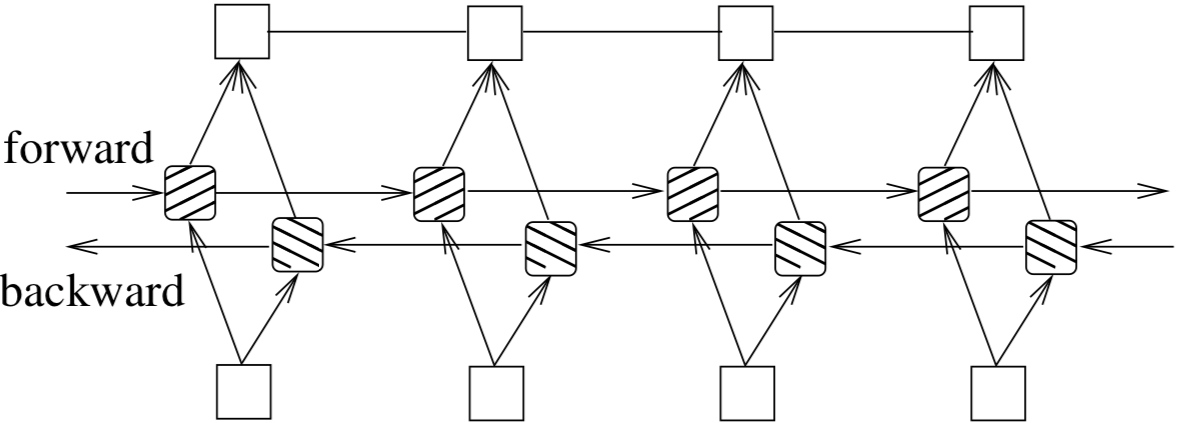
\includegraphics[width=0.6\linewidth]{bilstm.png}}
	\caption{Схема модели с BiLSTM.}
	\label{ris:image3}
\end{figure}

В рассматриваемой задаче очень важно знать не только предыдущий контекст, но и будущий. Такую возможность предоставляет BiLSTM \cite{Gers2000}, основная идея которой заключается в обработке каждой последовательности в прямом и обратном направлениях в двух отдельных слоях (рис.2). Для входного предложения $(\mathbf{w_1}, \mathbf{w_2}, \dots, \mathbf{w_n})$, содержащего $\mathbf{n}$ слов, слой LSTM вычисляет представление $\overrightarrow{\mathbf{h_i}}$ для каждого слова $\mathbf{w_{i}}$. Аналогично вычисляется $\overleftarrow{\mathbf{h_i}}$, для обратного предложения. В результате, BiLSTM путем конкатенации полученных двух представлений $\mathbf{h_i}=[\overrightarrow{\mathbf{h_i}},\overleftarrow{\mathbf{h_i}}]$ получает информацию о предыдущем и будущем контекстах слова.

\subsection{Условные случайные поля}
В задачах разметки последовательностей, в число которых входит рассматриваемая задача, очень важно понимать зависимости между смежными метками, т.е. нужно не допускать ситуации, когда метка \textsc{i-mut} возникает перед \textsc{b-mut} в пределах одной сущности или возникает сразу после \textsc{b-gene}. Это позволяют сделать такой класс дискриминативных статистических моделей, как условные случайные поля (рис.3) \cite{Sutton12anintroduction, Lafferty01conditionalrandom}.

На вход подается предложение $\mathbf{x}=\left(\mathit{x_1, x_2, \dots, x_n}\right)$. Оценка, отражающая правильность предсказанной последовательности меток, записывается следующим образом:
$$\mathit{s}\left(\mathbf{x},\mathbf{y}\right)=\sum_{t=1}^{n+1}\left(\mathbf{A}_{y_{t-1},y_t}+\mathbf{P}_{t, y_t}\right),$$
где 	$\mathbf{P}_{t, y_t}$ вычисляет оценку соответствия метки $\mathit{y_t}$ слову $\mathit{x_t}$ (в нашем случае $\mathbf{P}_{t, y_t}=\mathbf{W}_h\cdot\mathbf{h}+\mathbf{b}_h$), $\mathbf{A}$ -- матрица транзитивности (матрица вероятностей переходов от метки $y_{t-1}$ к $y_t$ на шаге $\mathit{t}$). Отметим, что в терминах CRF $\mathit{x_t}$ называются скрытыми состояниями, а $\mathit{y_t}$ -- наблюдаемыми.

\begin{figure}[h]
	\center{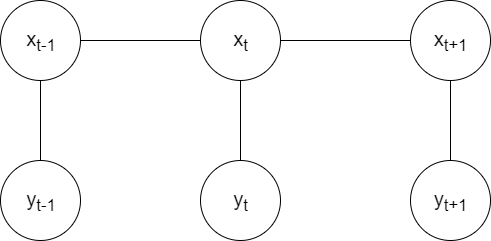
\includegraphics[width=0.5\linewidth]{crf.png}}
	\caption{Граф CRF на шаге $\mathit{t}$.}
	\label{ris:image4}
\end{figure}

Если учесть все возможные последовательности меток, то можно получить вероятность такой последовательности:
$$\mathbb{P}\{\mathbf{y}|\mathbf{x}\}=\frac{\prod_{n}\exp(\mathit{s}\left(\mathbf{x},\mathbf{y}\right))}{\sum_{\tilde{\mathbf{y}}\in\mathbf{Y}_{\mathbf{x}}}\prod_{n}\exp(\mathit{s}\left(\mathbf{x},\tilde{\mathbf{y}}\right))},$$
$\mathbf{Y}_{\mathbf{x}}$ -- все возможные последовательности меток в предложении $\mathbf{x}$.

Так как в процессе обучения максимизируется логарифм правдоподобия правильной последовательности меток, то
$$\log(\mathbb{P}\{\mathbf{y}|\mathbf{x}\}) = \mathit{s}\left(\mathbf{x},\mathbf{y}\right) - \log\left(\sum_{\tilde{\mathbf{y}}\in\mathbf{Y}_{\mathbf{x}}}\exp(\mathit{s}\left(\mathbf{x},\tilde{\mathbf{y}}\right))\right).$$

В процессе декодирования, наиболее вероятная последовательность меток $\mathit{y}^*$ соответствует максимальному значению оценки $\mathit{s}$: 
$$\mathit{y}^* = \underset{\tilde{\mathbf{y}}\in\mathbf{Y}_{\mathbf{x}}}{\text{argmax}} ~ \mathit{s}\left(\mathbf{x},\tilde{\mathbf{y}}\right)$$

\subsection{Модель GMNet}

Как было сказано выше, BiLSTM способна учитывать предыдущий и будущий контекст, а CRF способны предсказывать метки сушностей, учитывая их взаимосвязь с другими метками. Используя оба этих подхода, была разработана модель GMNet для решения рассматриваемой задачи поиска именованных сущностей генов и мутаций (рис.4).
\begin{figure}[h]
	\center{\includegraphics[width=0.8\linewidth]{GMNet.png}}
	\caption{Схематическая архитектура модели GMNet.}
	\label{ris:image5}
\end{figure}



Для обучения модели используются векторные представления слов, предобученные на научных медицинских статьях, взятых из ресурса PubMed \cite{pubmed}. Из этих слов формируется словарь $\mathbf{V}$. Так как рассматриваемая предметная область достаточно специфична и богата редкими словами, то часть из них будет не входить в словарь, и возникнет проблема OOV (out of vocabulary) слов. Для решения такой проблемы предлагается дополнительно обучать символьные эмбеддинги, из которых состоят слова. Очередное слово разделяется на отдельные символы, которые подаются на вход BiLSTM и добавляются в словарь $\mathbf{V}$. На выходе получаются эмбеддинги символов, которые конкатенируются к эмбеддингу слова, в которое они входят. Полученный вектор подается на вход BiLSTM, а её скрытые состояния подаются в CRF слой, который предсказывает метку текущего слова. 

Модель GMNet реализована на языке Python с помощью библиотеки для работы нейронными сетями PyTorch, включает 4128462 обучаемых параметров. Размерность эмбеддингов составляет 200, используется 2 BiLSTM слоя (под символы и слова) и 1 CRF слой. Для предотвращения переобучения применяется техника дропаут с вероятностью удаления связи 0.5. В качестве оптимизатора выбран стохастический градиентный спуск (SGD) со стартовым шагом $0.001$, умножающимся на $0.8$ каждую эпоху.


%%%%%%%%%%%%%%%%%%%%%%%%%%%%%%%%%%%%%%%%%%%%%%%%%%%%%


\newpage
\section{Вычислительный эксперимент}
В данном разделе описаны используемые в работе данные, параметры модели GMNet, а также анализ полученных результатов.

\subsection{Данные}
	Приведем краткий перечень основных источников данных для именованных сущностей генов и мутаций.
	
	\bigskip
	
	\textbf{Гены:}
	\begin{itemize}
		\item \textit{BC2GM} \cite{pmid15960837} ~--- объемный корпус, состоящий из 20к предложений и содержащий аннотации для именованных сущностей генов и белков.
		\item \textit{JNLPBA} \cite{Huang2019} ~--- корпус, состоящий из 22к предложений, содержащих информацию о названиях генов, белков и т.п. 
	\end{itemize}

	\bigskip
	
		\textbf{Мутации:}
	\begin{itemize}
		\item \textit{tmVar} \cite{pmid23564842} ~--- корпус, состоящий из 500 размеченных биомедицинских статей с аннотациями сущностей генных и белковых мутаций. 
		\item \textit{MutationFinder} \cite{pmid27256315} ~--- корпус, включающий в себя предложения из медицинских научных статей с размеченными человеческими мутациями.
	\end{itemize}

На основе выше перечисленных наборов данных был составлен корпус для обучения модели GMNet. Объем обучающей выборки ~-- 40к, валидационной ~-- 5.7к, тестовой ~-- 11.4к. Обработанные данные представляют собой набор строк вида $\left(token, tag\right)$, где $token\in V$ и $tag\in \left[\textsc{o, b-gene, i-gene, b-mut, i-mut}\right]$. 


\bigskip

Ниже приведена таблица 1, содержащая информацию о собранных наборах данных.
\begin{center}
	 
	\begin{table}[h]
		\centering
		Таблица 1. Наборы данных
		%\begin{tabular}{l|l|l|l}
		\begin{tabular}{cccc}
			\hline Корпус & Кол-во генов & Кол-во мутаций & Кол-во предложений\\
			\hline JNLPBA & 10589 & - & 22562\\
			BC2GM & 24583 & - & 20510\\
			\hline
			MutationFinder & - & 5611 & 8176\\
			tmVar & - & 3702 & 5956\\
			\hline 
		\end{tabular}
		\label{Tab:2}
	\end{table}
\end{center}

Можно заметить, что общее число сущностей мутаций меньше числа сущностей генов приблизительно в четыре раза. Соответственно, классы несбалансированы. Для решения этой проблемы используется метод, описанный в \cite{Padurariu2019}. Применяется техника \textit{oversampling}, что означает случайное добавление экземпляров <<слабого>> класса в выборку. 

\bigskip

Ниже приведены примеры <<сложных>> и <<простых>> сущностей из данных.
\textit{Many \underline{erythroid cell-specific genes}, including \underline{alpha and beta-globin.}}
\\
\textit{Mouse \underline{interleukin-2 receptor alpha gene} expression.}
\\
\textit{The \underline{-491 A to T} substitution decreased the activity.}
\\
\textit{A novel heterozygous \underline{c.3703T>C} change in exon.}

Стоит отметить, что наибольшую трудность в поиске оказывают сущности, записанные на естественном языке (первый и второй примеры).
\subsection{Эксперимент}
Нейронная сеть GMNet обучалась 15 эпох. Ниже представлены результаты обучения.

\begin{figure}[h]
	\center{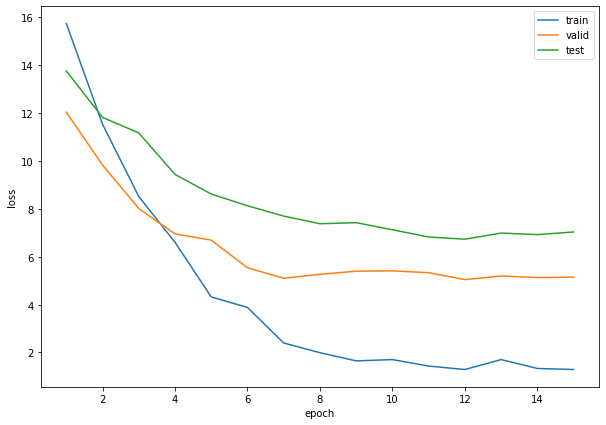
\includegraphics[width=0.7\linewidth]{final_loss.png}}
	\caption{График зависимости функции ошибки от числа эпох. Синий цвет соответствует обучающей выборке, оранжевый -- валидационной, зелёный -- тестовой.}
	\label{ris:image7}
\end{figure}

Из рисунка 6 видно, что модель сходится, переобучения не наблюдается.
\\
\\
\\

\begin{figure}[h]
	\center{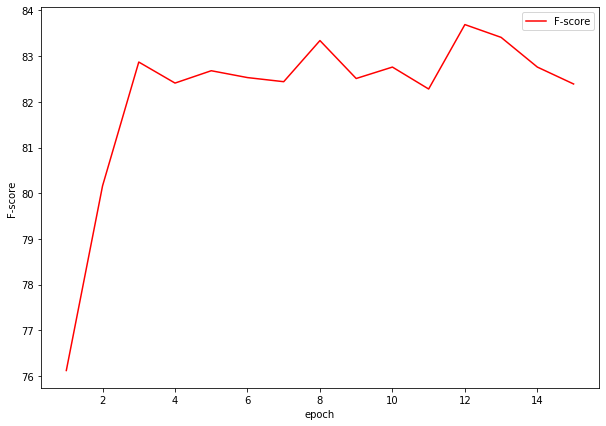
\includegraphics[width=0.7\linewidth]{final_f.png}}
	\caption{График зависимости F-меры от числа эпох на тестовой выборке.}
	\label{ris:image6}
\end{figure}

Из рисунка 7 видно, что лучший результат модель демонстрирует на 12 эпохе, далее значение показателя качества начинает снижаться и больше не достигает наилучшего результата.

В таблицах 2 и 3 содержатся значения полученных метрик \textit{Precision, Recall, F-score} предлагаемой модели GMNet, а также существующих моделей, демонстрирующих лучшие результаты в решении рассматриваемой задачи.
 


\begin{center}
	\begin{table}[h]
		\centering
		Таблица 2 и 3. Результаты для сущностей генов и мутаций.
		\begin{tabular}{cccc}
			\hline Модель & Precision &  Recall & F-score \\
			\hline Collabonet & 79.70 & 77.47 & 78.56 \\
			BioBERT & 84.32 & 85.12 & 84.72 \\
			Wang et al. 2018 & 81.11 & 78.91 & 80.00 \\
			\hline
			\textbf{GMNet}&   \textbf{81.59}&   \textbf{79.13} & \textbf{80.34}   \\
			\hline 
		\end{tabular}
		\label{Tab:1}
	\end{table}
	
	\begin{table}[h]
		\centering
		\begin{tabular}{cccc}
			\hline Модель & Precision &  Recall & F-score \\
			\hline tmVar & 94.96 & 79.01 & 86.25 \\
			nala & 86.32 & 92.20 & 89.16 \\
			SETH & 96.42 & 74.66 & 84.15 \\
			\hline
			\textbf{GMNet} & \textbf{87.71}& \textbf{86.48} & \textbf{87.09}   \\
			\hline 
		\end{tabular}
		\label{Tab:3}
	\end{table}
\end{center}

Видно, что результаты получились соизмеримыми с результатами существующих решений, что говорит о состоятельности модели GMNet.

\subsection{Анализ результатов}
Рассмотрим полученные результаты на тестовой выборке. Примеры размеченных моделью предложений в сравнении с правильной разметкой приведены на рисунке 8.

\begin{figure}[h]
	\center{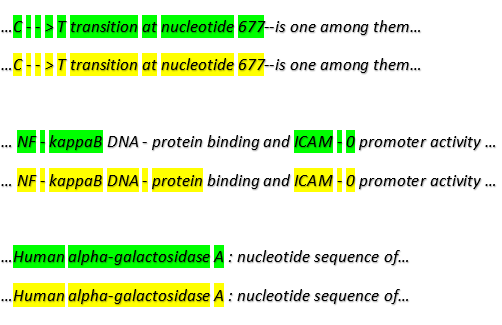
\includegraphics[width=0.7\linewidth]{results.png}}
	\label{ris:image8}
\end{figure}
\begin{figure}[h]
	\center{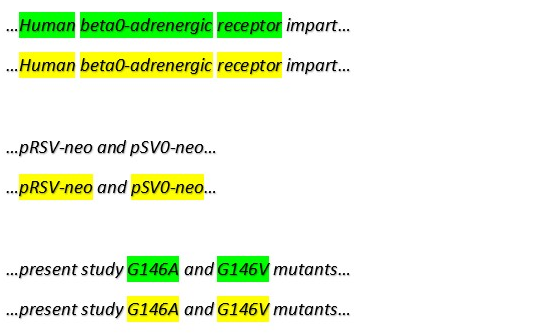
\includegraphics[width=0.7\linewidth]{results2.png}}
	\caption{Результаты работы GMNet на тестовой выборке. Зеленым обозначена верная разметка, желтым - предсказание модели.}
	\label{ris:image9}
\end{figure}


Как можно заметить, модель достаточно хорошо научилась находить именованные сущности генов и мутаций. Но возникают небольшие коллизии, как показано на рис.8. Видно, что модель нашла лишнюю часть в сущности гена \textit{NF-kappaB}. Произошло это, скорее всего, из-за того, что очень часто рядом со связкой слов \textit{DNA-Protein} возникали названия генов. Но даже такая разметка уже дает ценную информацию о гене.
Также можно заметить, что редко модель выделяет сущность там, где её на самом деле нет.
%%%%%%%%%%%%%%%%%%%%%%%%%%%%%%%%%%%%%%%%%%%%%%%%%%%%%


\newpage
\section{Заключение}

Была решена задача извлечения именованных сущностей генов и мутаций из биомедицинских текстов с помощью подходов глубокого обучения и использования контекстной информации отдельных сущносетй. Модель показала высокие результаты, сравнимые с уже существующими решениями. В дальнейших исследованиях предлагается:

\begin{enumerate}
	\item использовать дополнительную информацию на уровне n-gramm;
	\item использовать дополнительные признаки, такие как часть речи и регистр токена;
	\item реализовать в модели механизм внимания.
\end{enumerate}

%%%%%%%%%%%%%%%%%%%%%%%%%%%%%%%%%%%%%%%%%%%%%%%%%%%%%


\newpage
\bibliographystyle{gost71s}
\bibliography{mylib}


\end{document}